\documentclass[a4paper,12pt,twoside]{memoir}

% Castellano
\usepackage[spanish,es-tabla]{babel}
\selectlanguage{spanish}
\usepackage[utf8]{inputenc}
\usepackage[T1]{fontenc}
\usepackage{lmodern} % scalable font
\usepackage{microtype}
\usepackage{placeins}

\RequirePackage{booktabs}
\RequirePackage[table]{xcolor}
\RequirePackage{xtab}
\RequirePackage{multirow}

% Links
\usepackage[colorlinks]{hyperref}
\hypersetup{
	allcolors = {red}
}

% Ecuaciones
\usepackage{amsmath}

% Rutas de fichero / paquete
\newcommand{\ruta}[1]{{\sffamily #1}}

% Párrafos
\nonzeroparskip


% Imagenes
\usepackage{graphicx}
\newcommand{\imagen}[2]{
	\begin{figure}[!h]
		\centering
		\includegraphics[width=0.9\textwidth]{#1}
		\caption{#2}\label{fig:#1}
	\end{figure}
	\FloatBarrier
}

\newcommand{\imagenflotante}[2]{
	\begin{figure}%[!h]
		\centering
		\includegraphics[width=0.9\textwidth]{#1}
		\caption{#2}\label{fig:#1}
	\end{figure}
}



% El comando \figura nos permite insertar figuras comodamente, y utilizando
% siempre el mismo formato. Los parametros son:
% 1 -> Porcentaje del ancho de página que ocupará la figura (de 0 a 1)
% 2 --> Fichero de la imagen
% 3 --> Texto a pie de imagen
% 4 --> Etiqueta (label) para referencias
% 5 --> Opciones que queramos pasarle al \includegraphics
% 6 --> Opciones de posicionamiento a pasarle a \begin{figure}
\newcommand{\figuraConPosicion}[6]{%
  \setlength{\anchoFloat}{#1\textwidth}%
  \addtolength{\anchoFloat}{-4\fboxsep}%
  \setlength{\anchoFigura}{\anchoFloat}%
  \begin{figure}[#6]
    \begin{center}%
      \Ovalbox{%
        \begin{minipage}{\anchoFloat}%
          \begin{center}%
            \includegraphics[width=\anchoFigura,#5]{#2}%
            \caption{#3}%
            \label{#4}%
          \end{center}%
        \end{minipage}
      }%
    \end{center}%
  \end{figure}%
}

%
% Comando para incluir imágenes en formato apaisado (sin marco).
\newcommand{\figuraApaisadaSinMarco}[5]{%
  \begin{figure}%
    \begin{center}%
    \includegraphics[angle=90,height=#1\textheight,#5]{#2}%
    \caption{#3}%
    \label{#4}%
    \end{center}%
  \end{figure}%
}
% Para las tablas
\newcommand{\otoprule}{\midrule [\heavyrulewidth]}
%
% Nuevo comando para tablas pequeñas (menos de una página).
\newcommand{\tablaSmall}[5]{%
 \begin{table}
  \begin{center}
   \rowcolors {2}{gray!35}{}
   \begin{tabular}{#2}
    \toprule
    #4
    \otoprule
    #5
    \bottomrule
   \end{tabular}
   \caption{#1}
   \label{tabla:#3}
  \end{center}
 \end{table}
}

%
%Para el float H de tablaSmallSinColores
\usepackage{float}

%
% Nuevo comando para tablas pequeñas (menos de una página).
\newcommand{\tablaSmallSinColores}[5]{%
 \begin{table}[H]
  \begin{center}
   \begin{tabular}{#2}
    \toprule
    #4
    \otoprule
    #5
    \bottomrule
   \end{tabular}
   \caption{#1}
   \label{tabla:#3}
  \end{center}
 \end{table}
}

\newcommand{\tablaApaisadaSmall}[5]{%
\begin{landscape}
  \begin{table}
   \begin{center}
    \rowcolors {2}{gray!35}{}
    \begin{tabular}{#2}
     \toprule
     #4
     \otoprule
     #5
     \bottomrule
    \end{tabular}
    \caption{#1}
    \label{tabla:#3}
   \end{center}
  \end{table}
\end{landscape}
}

%
% Nuevo comando para tablas grandes con cabecera y filas alternas coloreadas en gris.
\newcommand{\tabla}[6]{%
  \begin{center}
    \tablefirsthead{
      \toprule
      #5
      \otoprule
    }
    \tablehead{
      \multicolumn{#3}{l}{\small\sl continúa desde la página anterior}\\
      \toprule
      #5
      \otoprule
    }
    \tabletail{
      \hline
      \multicolumn{#3}{r}{\small\sl continúa en la página siguiente}\\
    }
    \tablelasttail{
      \hline
    }
    \bottomcaption{#1}
    \rowcolors {2}{gray!35}{}
    \begin{xtabular}{#2}
      #6
      \bottomrule
    \end{xtabular}
    \label{tabla:#4}
  \end{center}
}

%
% Nuevo comando para tablas grandes con cabecera.
\newcommand{\tablaSinColores}[6]{%
  \begin{center}
    \tablefirsthead{
      \toprule
      #5
      \otoprule
    }
    \tablehead{
      \multicolumn{#3}{l}{\small\sl continúa desde la página anterior}\\
      \toprule
      #5
      \otoprule
    }
    \tabletail{
      \hline
      \multicolumn{#3}{r}{\small\sl continúa en la página siguiente}\\
    }
    \tablelasttail{
      \hline
    }
    \bottomcaption{#1}
    \begin{xtabular}{#2}
      #6
      \bottomrule
    \end{xtabular}
    \label{tabla:#4}
  \end{center}
}

%
% Nuevo comando para tablas grandes sin cabecera.
\newcommand{\tablaSinCabecera}[5]{%
  \begin{center}
    \tablefirsthead{
      \toprule
    }
    \tablehead{
      \multicolumn{#3}{l}{\small\sl continúa desde la página anterior}\\
      \hline
    }
    \tabletail{
      \hline
      \multicolumn{#3}{r}{\small\sl continúa en la página siguiente}\\
    }
    \tablelasttail{
      \hline
    }
    \bottomcaption{#1}
  \begin{xtabular}{#2}
    #5
   \bottomrule
  \end{xtabular}
  \label{tabla:#4}
  \end{center}
}



\definecolor{cgoLight}{HTML}{EEEEEE}
\definecolor{cgoExtralight}{HTML}{FFFFFF}

%
% Nuevo comando para tablas grandes sin cabecera.
\newcommand{\tablaSinCabeceraConBandas}[5]{%
  \begin{center}
    \tablefirsthead{
      \toprule
    }
    \tablehead{
      \multicolumn{#3}{l}{\small\sl continúa desde la página anterior}\\
      \hline
    }
    \tabletail{
      \hline
      \multicolumn{#3}{r}{\small\sl continúa en la página siguiente}\\
    }
    \tablelasttail{
      \hline
    }
    \bottomcaption{#1}
    \rowcolors[]{1}{cgoExtralight}{cgoLight}

  \begin{xtabular}{#2}
    #5
   \bottomrule
  \end{xtabular}
  \label{tabla:#4}
  \end{center}
}




\graphicspath{ {./img/} }

% Capítulos
\chapterstyle{bianchi}
\newcommand{\capitulo}[2]{
	\setcounter{chapter}{#1}
	\setcounter{section}{0}
	\chapter*{#2}
	\addcontentsline{toc}{chapter}{#2}
	\markboth{#2}{#2}
}

% Apéndices
\renewcommand{\appendixname}{Apéndice}
\renewcommand*\cftappendixname{\appendixname}

\newcommand{\apendice}[1]{
	%\renewcommand{\thechapter}{A}
	\chapter{#1}
}

\renewcommand*\cftappendixname{\appendixname\ }

% Formato de portada
\makeatletter
\usepackage{xcolor}
\newcommand{\tutor}[1]{\def\@tutor{#1}}
\newcommand{\course}[1]{\def\@course{#1}}
\definecolor{cpardoBox}{HTML}{E6E6FF}
\def\maketitle{
  \null
  \thispagestyle{empty}
  % Cabecera ----------------
\noindent
\includegraphics[width=\textwidth]{cabecera}\vspace{1cm}%
  \vfill
  % Título proyecto y escudo informática ----------------
  \colorbox{cpardoBox}{%
    \begin{minipage}{.8\textwidth}
      \vspace{.5cm}\Large
      \begin{center}
      \textbf{TFG del Grado en Ingeniería Informática}\vspace{.6cm}\\
      \textbf{\LARGE\@title{}}
      \end{center}
      \vspace{.2cm}
    \end{minipage}

  }%
  \hfill\begin{minipage}{.20\textwidth}
    
\includegraphics[width=\textwidth]{escudoInfor}
  \end{minipage}
  \vfill
  % Datos de alumno, curso y tutores ------------------
  \begin{center}%
  {%
    \noindent\LARGE
    Presentado por \@author{}\\ 
    en Universidad de Burgos --- \@date{}\\
    Tutor: \@tutor{}\\
  }%
  \end{center}%
  \null
  \cleardoublepage
  }
\makeatother


% Datos de portada
\title{título del TFG \\Documentación Técnica}
\author{nombre alumno}
\tutor{nombre tutor}
\date{\today}

\begin{document}

\maketitle



\cleardoublepage



%%%%%%%%%%%%%%%%%%%%%%%%%%%%%%%%%%%%%%%%%%%%%%%%%%%%%%%%%%%%%%%%%%%%%%%%%%%%%%%%%%%%%%%%



\frontmatter


\clearpage

% Indices
\tableofcontents

\clearpage

\listoffigures

\clearpage

\listoftables

\clearpage

\mainmatter

\appendix

\apendice{Plan de Proyecto Software}

\section{Introducción}

En este apartado se tratarán varios temas importantes a la hora de realizar un trabajo. 

Uno de ellos será la planificación temporal, a través de la cual se sabrá la asignación de tiempos que realizar durante todo el trascurso del proyecto.

Todo el trabajo se desarrolla en torno a metodologías de trabajo como SCRUM, con la cual se puede conseguir una identificación mas sencilla de la asignación de tareas y tiempos y la inversión de tiempo en proporción al total de horas que llevará el proyecto.

Otro es el estudio de la viabilidad, donde se tratarán dos puntos esenciales, la viabilidad económica y la viabilidad legal. Por la parte económica se tratará de simular las consecuencias que conlleva manejar unas herramientas u otras a la hora de invertir dinero en el proyecto o de que otras personas vayan a invertirlo cuando se trate venderlo.

La viabilidad legal se centrará un poco más en el estudio de los derechos de copyright, así como el trato que se haga de los datos. Por último también se tendrá en cuenta la seguridad en cuando a protección de los datos y las capas de seguridad del sistema que tratamos.

\section{Planificación temporal}

El objetivo inicial al planificar un proyecto es definir lo más claro posible el marco de tiempo y de recursos que se llevarán a cabo durante el desarrollo del proyecto. Como ya mencionábamos antes, se basa en la metodología SCRUM.

Dado que este proyecto ha sufrido bastantes cambios sobre la planificación y desarrollo del mismo desde que se comenzó hasta la actualidad, haremos una comparación entre lo que inicialmente se planeó y lo que finalmente resulta, a fin de poder ver todo lo que un trabajo como este, donde no se definen unos objetivos claros desde un inicio, o se definen objetivos sin planificar las consecuencias puede variar y evolucionar.

El proyecto comienza el día 5 de abril de 2019 y finaliza el día 13 de febrero de 2020, con una duración bruta de 10 meses. Ésta duración también se debe, como se ha mencionado antes, a los cambios que ha ido sufriendo el desarrollo del proyecto. Igualmente, también hay que tener en cuenta que no se ha dedicado todo el tiempo a la realización del proyecto, ya que también era necesario aprobar las asignaturas restantes así como realizar prácticas laborales durante todo este período. También se terminó aplazando la entrega debido a la imposibilidad de presentar en la convocatoria de Septiembre por no cumplir los requisitos de créditos máximos presentables en la misma.

Por todo esto que se expone, la realización del proyecto ha tenido una evolución irregular, con meses más activos que otros debido a la complicación para realizar reuniones entre los tutores y los alumnos participantes del mismo.

Se pueden ver las partes que ha conllevado:

\begin{itemize}

\item SCRUM se basa en la división de las tareas y recursos en intervalos de tiempo, por lo que será como se desarrolle. 

\item Cada uno de los sprints conllevará unas tareas a realizar durante ese intervalo. Se trató de que las reuniones se realizaran cada 2 semanas, o una vez al mes.

\end{itemize}

El comienzo del proyecto se realizó con una reunión estándar con el tutor, que nos comentó el punto de partida y los objetivos iniciales que podríamos tener para comenzar el trabajo.

Cabe destacar que se explicará cada uno de los sprints partiendo siempre de una reunión inicial, y estableciendo las nuevas tareas que se realizarán durante el mismo.

\subsection{Sprint 1 (05/04/19 - 19/04/19)}

En esta primera reunión el tutor explica los objetivos iniciales y se establecen las siguientes tareas:

\begin{itemize}
\item Búsqueda de documentación sobre Android.
\item Desarrollo de objetivos iniciales de cara a la memoria.
\item Consulta inicial del proyecto base del que partíamos.
\end{itemize}

\subsection{Sprint 2 (19/04/19 - 03/05/19)}

Tras el primer sprint, pudimos comentar el conocimiento que cada uno tenía sobre la plataforma sobre la que trabajaríamos así como el lenguaje de programación. En mi caso, nunca había utilizado el programa de Android Studio ni programado para un entorno Android, aunque si que conocía el lenguaje de programación Java.

Se propuso lo siguiente:

\begin{itemize}
\item Comenzar a nutrirse de tutoriales y vídeos explicativos sobre Android.
\item Instalar la herramienta de Android Studio.
\item Pensar en la viabilidad de actualizar la versión en la que se encuentra el proyecto, así como las posibilidades de cambiar de herramienta de desarrollo, porque en ese momento el proyecto se había desarrollado en Eclipse, con un plugin para Android debido a la inexistencia de Android Studio en esa época.
\end{itemize}

\subsection{Sprint 3 (03/05/19 - 17/05/19)}

En este encuentro, se trata las posibilidades de lo comentado en la reunión anterior, concluyendo que el cambio de herramienta de desarrollo será algo positivo y relativamente fácil de hacer, pero sin tener claro las posibilidades sobre la actualización de versiones. 

Se trata de desarrollar lo siguiente para el siguiente sprint:

\begin{itemize}
\item En caso de plantear la actualización, buscar la versión actual más óptima hacia la que se debería hacer, para evitar versiones inestables y con bugs.
\item Instalar el proyecto inicial a través de maquinas virtuales y probar todas las funcionalidades que contiene, para conocer bien sobre lo que vamos a trabajar.
\item Seguir desarrollando apartados referentes de la memoria para ir quitando carga de trabajo al final.
\end{itemize}

\subsection{Sprint 4 (17/05/19 - 07/06/19)}

En esta reunión, tras tratar los temas anteriores, se concluye que la versión a la que actualizar debe ser Android 6.0 (API 23), viniendo desde android 4.4 (API 14). Supone un gran salto pero si queremos que la aplicación sea funcional con la tecnología de hoy en día habrá que usar una versión viable. Sobre este tema se plantea el hecho de la antigüedad del proyecto, teniendo en cuenta esto para el resto del desarrollo.

Se intenta realizar lo siguiente:

\begin{itemize}
\item Instalación del proyecto base sobre la nueva herramienta de desarrollo, para intentar que este quede ya funcional en Android Studio.
\item Documentación sobre cambios de versiones en Android hasta la versión sobre la que se desarrolla.
\end{itemize}

\subsection{Sprint 5 (07/06/19 - 05/07/19)}

Reunión cercana a los meses de verano, por lo que se intenta dejar objetivos más a largo plazo, aunque también comentando las dificultades que se van encontrando a la hora de instalar y hacer que funcione el proyecto sobre la nueva herramienta:

\begin{itemize}
\item Conseguir que definitivamente la aplicación alcance un estado de funcionamiento correcto sobre Android Studio.
\item Aplicar el cambio de versión sobre el proyecto y por consiguiente comenzar a solucionar todos los errores de base que se encuentren.
\end{itemize}

\subsection{Sprint 6 (05/07/19 - 03/09/19)}

En esta reunión, tras observar los problemas que supone hacer que funcione la aplicación sobre Android Studio y por consiguiente actualizarla, los objetivos de la anterior reunión siguen siendo los mismos con algunos añadidos.

El problema principal parece ser que la gran mayoría de librerías que se utilizaron en el proyecto inicial han dejado de tener soporte y han dejado de funcionar, por lo que todo ese código es ahora inservible y habrá que buscar una sustitución.

Se plantean los objetivos anteriores añadiendo:

\begin{itemize}
\item Desarrollo de la memoria, tratando de quitar carga a futuro.
\item Arreglo de errores con bibliotecas.
\item Documentación sobre nuevas APIs utilizables para sustituir todas las que ya están obsoletas.
\end{itemize}

\subsection{Sprint 7 (03/09/19 - 04/11/19)}

Una reunión tratando de ver los avances del verano, para después poner objetivos a largo plazo. En este momento ya se presentan más dificultades para trabajar en el proyecto y tener reuniones habituales por diversos motivos.

A partir de los objetivos que se tenían inicialmente, se intenta establecer unos más realistas teniendo en cuenta la situación:

\begin{itemize}
\item Continuar con todos los arreglos necesarios sobre la aplicación, ya que según se van solucionando algunas incompatibilidades, se van descubriendo nuevas.
\item Intentar continuar el desarrollo de la memoria.
\end{itemize}

\subsection{Sprint 8 (04/11/19 - 18/11/19)}

Tras el tiempo que ha pasado, se intenta tener un seguimiento sobre las tareas que habían sido asignadas. Por desgracia, estas tareas no varían demasiado, ya que supone un trabajo importante la documentación sobre los métodos que tienen que ser sustituidos para incluir otro nuevos, sobre los que también es necesario documentarse previamente, sobre un lenguaje de programación relativamente nuevo.

\subsection{Sprint 9 (18/11/19 - 02/12/19)}

Tras haber ido trabajando, en esta nueva reunión se presenta un problema que ha ido siendo recurrente durante el desarrollo del proyecto, ya que aunque se han solucionado muchos problemas, la conexión entre la parte del cliente y la del servidor no parece funcionar, lo cual genera bastante incertidumbre porque se desconoce si la causa puede venir desde el cliente o desde el servidor y este problema se va arrastrando.

Objetivos anteriores añadiendo:

\begin{itemize}
\item Tratar de arreglar el problema de la conexión, identificando el origen y tratándolo.
\end{itemize}

\subsection{Sprint 10 (02/12/19 - 16/12/19)}

Reunión sin demasiado contenido, ya que se sigue tratando de realizar las mismas tareas, por lo que los objetivos que ya se tenían, se trasladan a este sprint.

\subsection{Sprint 11 (16/12/19 - 13/01/20)}

Una de las ultimas reuniones que se producen, tratando de ver los últimos objetivos que se tienen de cara a finalizar el trabajo, así como viendo si es posible arreglar la conexión. 

Se detectan varios problemas que pueden llegar a ser la causa, aparte de la diferencia de versiones entre la aplicación y el servidor que, a la hora de comunicarse generan problemas.

\begin{itemize}
\item Tratándose de fechas cercanas a la entrega, desarrollar la memoria.
\item Solucionar conexión.
\item Depurar el código.
\item Cambios visuales propuestos sobre la aplicación para mejorar la accesibilidad de la misma.
\end{itemize}

\subsection{Sprint 12 (13/01/20 - 07/02/20)}

En esta reunión se establece los últimos objetivos, así como una fecha para entregar la memoria a los tutores para que puedan revisarla y proponer mejoras.

\begin{itemize}
\item Continuar depurando código.
\item Finalizar memoria.
\end{itemize}

\subsection{Sprint 13 (07/02/20 - Fin de proyecto)}

Para la última reunión se proponen cambios en la memoria y se realiza una visión general sobre el proyecto.

\begin{itemize}
\item Finalizar código.
\item Realizar mejoras en memoria.
\item Pancarta.
\end{itemize}


Ya se ha visto que el trascurso de este proyecto ha tenido épocas más activas que otras, debido a las complicaciones que se comentan. De todas formas se ha tratado de seguir la metodología de la mejor manera posible.

\section{Estudio de viabilidad}

Como ya hemos comentado antes, en este apartado se trata la viabilidad del proyecto, de manera económica y legal, ya que cabe la posibilidad de que un proyecto posea las cualidades para ser interesante de realizar, pero no ser viable económicamente o legalmente debido a protección de ciertos u otros factores.

Hay otro factor, que en el caso concreto de este proyecto adquiere mucha importancia, que es la viabilidad de realizar el proyecto a nivel de magnitud y conocimiento. Lo trataremos inicialmente:

\subsection{Viabilidad sobre la magnitud y conocimiento del proyecto}

Hay que tener en cuenta una serie de factores en este apartado:

\begin{itemize}

\item Conocimiento sobre el lenguaje que se va a utilizar.
\item Conocimiento sobre la herramienta que se va a utilizar.
\item Análisis sobre la viabilidad de desarrollo del proyecto en cuestión, estableciendo límites de tiempos y recursos.
	
	Con respecto a esta parte, es algo que a la hora de planificar un proyecto hay que tener muy en cuenta, porque aunque pueda resultar algo muy interesante, puede no ser viable debido a la complejidad del mismo.
	
	En nuestro caso, si se hubiera realizado de forma más minuciosa este apartado, probablemente se habría llegado a la conclusión de que es un proyecto de final de carrera muy poco viable, porque supone obtener conocimiento sobre herramientas y lenguajes nunca utilizados, analisis de un codigo que no es propio, desarrollado en versiones con mas de 7 años de antigüedad, tratar de actualizarlo sin conocer perfectamente todas las dificultades que se pueden encontrar, etc.
	
	Por todo lo mencionado se plantea este apartado, para que una persona que comience un proyecto, trate minuciosamente la información de la que dispone, y analice las ventajas e inconvenientes que supone, así como el tiempo del que dispondrá para su desarrollo.

\end{itemize}



\subsection{Viabilidad económica}

Dado que partimos de un proyecto anterior, es conveniente mencionarlo, ya que en él se realiza un análisis sobre la viabilidad económica bastante acertado y que contiene información perfectamente válida para el estudio de la viabilidad de nuestro proyecto.

\subsubsection{Análisis de costes}

Tal como se menciona en el proyecto anterior, tendremos en cuenta 4 tipos de costes:

\begin{itemize}
\item Coste de personal
\end{itemize}

La persona que se encargará de realizar el proyecto será un desarrollador de software, y como hemos comentado que el proyecto tiene una duración de unos 10 meses, con una media de 4 horas diarias trabajadas tendremos una estimación bastante decente, con épocas mas activas y otras menos. En este caso tomaremos de referencia coste/hora del proyecto anterior que suponía 12 euros/hora.

12 euros/hora trabajando 4 horas/día ---> 48 euros/Día

48 euros/día trabajando 5 días/semana ---> 240 euros/semana

240 euros/semana trabajando 4 semanas/mes ---> 960 euros/mes

Al estimar este proyecto en 10 meses, el coste por el desarrollador sería:

960 euros/mes trabajando 10 meses ---> \textbf{9600 euros brutos}.

Este sueldo se corresponde con el sueldo bruto del trabajador que percibe de la empresa. A esto, le tenemos que descontar la cotización al a Seguridad Social, que consultando en la propia Seguridad Social se calcula un 23.6 \% por contingencias comunes, un 7.7 \% en concepto de desempleo en contrato de duración determinada a tiempo parcial y un 0.1 \% en concepto de formación profesional. Todo ello, hace un total de 31.4 \%

31.4 \% de 9600 = 3014,4 euros

Esto hace un total de 12,614,4 euros como coste del desarrollador.

\begin{itemize}
\item Coste HardWare
\end{itemize}

El coste del ordenador (HP Omen 15) que se ha utilizado está estimado en 1200 euros y el del móvil (BQ Aquaris E5)que se ha usado para hacer pruebas es de 150 euros. Cabe destacar que el uso de estos componentes no será exclusivo de este proyecto en particular, si no que se utilizarán fuera del ámbito del proyecto, por lo que estos costes son amortizables.


\begin{itemize}
\item Coste SoftWare
\end{itemize}

De todos los programas y software que ha sido utilizado, el único que se considera de pago es el sistema operativo, que es Windows 10, por lo que como coste Software habrá que añadir 145 euros del coste de la licencia de Windows Home.

Por último también hay que considerar otros costes:
\begin{itemize}
\item \textbf{Alquiler Oficina:} 250 euros/mes durante 10 meses ---> 2500 euros
\item \textbf{Material de oficina} 5 euros/mes durante 10 meses ---> 50 euros
\item \textbf{Impresión y encuadernación proyecto} 70 euros
\item \textbf{Electricidad} 30 euros/mes durante 10 meses ---> 300 euros
\item \textbf{Internet} 30 euros/mes durante 10 meses ---> 300 euros
\end{itemize}

\textbf{Total de gastos generales:} 2950 euros.

\begin{itemize}
\item Costes totales
\end{itemize}

Tras sumar todos los costes que tendríamos a lo largo del proyecto:

\textit{Coste total = coste personal + coste hardware + coste software + costes generales}

\textit{Coste total} = \textbf{17.059,4 euros}


\subsubsection{Análisis de costes/beneficios}

En este caso, es una buena opción adoptar las ideas representadas en los dos proyectos anteriores a este \cite{tfg1} \cite{tfm1}.

La idea que se propuso en la anterior versión del proyecto es que los negocios o establecimientos paguen una cuota fija anual, puesto que desde la aplicación van a mostrarse una serie de establecimientos recomendados para una ubicación determinada, y estos serán seleccionados de entre un conjunto, habitualmente grande, de negocios o establecimientos.

Mediante el pago de esa cuota, se potenciaría la frecuencia de aparición para ese establecimiento, de modo que para una consulta de un determinado usuario, cerca del susodicho establecimiento, éste aparecería como punto de interés en la ruta.

Se dará la posibilidad a los establecimientos de potenciar su frecuencia de aparición, para ello se ofrecen tres planes:

\begin{itemize}
\item \textbf{Standard:} 50 euros
\item \textbf{Premium:} 100 euros
\item \textbf{Golden:} 150 euros
\end{itemize}

La idea, aparte de este pago de cuotas, sería la de que la aplicación sea gratuita en Google Play Store, pero añadiendo posibilidad de descargar mapas pagando. Para ello se ofrecen tres maneras de descarga de mapas:

\begin{itemize}
\item \textbf{Gratuita:} Gratis y descarga de un mapa.
\item \textbf{Un único mapa:} descarga de un mapa adicional por 0.89 euros
\item \textbf{Pack de mapas:} descarga de todos los mapas de un país por 5.99 euros
\end{itemize}

Por último, también se plantea como una idea adicional añadir publicidad en la aplicación, para que el usuario por el simple hecho de estar usando la aplicación de forma gratuita, esté generando dinero de forma pasiva. Esta técnica es algo que hoy en día se ha normalizado por lo que no supondría una molestia excesiva a ningún usuario, mientras que es una manera sencilla de obtener beneficios.

\subsection{Viabilidad legal}

Para la viabilidad legal del proyecto, nos tendremos que fijar en la utilización de los datos y las licencias que se utilicen para desarrollar el trabajo.

Tal como se menciona aquí \cite{terminos}, para poder utilizar todas las funcionalidades que se nos ofrecen debemos aceptar ciertas condiciones y hacer un uso responsable de las mismas, para no infringir causas legales.

Para ello, dentro del propio proyecto desarrollado en Android Studio contaremos con archivos que harán referencia a estas licencias, y que todo proyecto que se desarrolle con estas tecnologías deberá incluir como parte de su estructura.



\apendice{Especificación de Requisitos}

\section{Introducción}

En este anexo contemplaremos varios aspectos, donde tenemos que tener en cuenta lo que quiere conseguir el cliente de este proyecto y lo que comprende el desarrollado sobre el mismo, para que todo le mundo acabe con una visión general lo más parecida posible. De esta forma evitaremos posibles decepciones por parte del cliente o demasiado trabajo para el programador en cuestión. Recogeremos una serie de aspectos que resultan muy relevantes a la hora de diseñar, entender y ejecutar un proyecto. Si esta parte queda bien definida entre la figura del desarrollador y la figura del cliente, el resto resultará mucho más fácil para ambos.

El objetivo principal es realizar un análisis del sistema que se va a desarrollar. Para ello, se definirán gráficos y diagramas donde se especifiquen los requisitos y requerimientos generales de nuestro proyecto. También es necesario definir las funciones que incorporaremos y las limitaciones que tendrá el sistema. Con respecto a estos dos últimos términos, cabe destacar que este trabajo se centrará más en actualización, optimización y mejora de la aplicación y no tanto en el desarrollo de funcionalidades, aunque si que habrá ciertas funcionalidades que se verán afectadas.

Se ayuda de elementos gráficos para poder visualizar la información sin tener que tener un conocimiento técnico elevado y donde se podrán ver los requisitos generales del sistema, así como las funciones que debería cumplir.

Por último también se incluirá una especificación de los requisitos mediante diagramas de casos de uso, donde de nuevo surgirán algunas modificaciones sobre funcionalidades ya existentes.

\section{Objetivos generales}

Los objetivo que definiremos para nuestro sistema serán los siguientes:

\begin{itemize}
\item Dado que contamos con una aplicación desarrollada para sistemas ya obsoletos, nuestro objetivo principal será el de conseguir que pueda funcionar dentro de un dispositivo actual.
	\begin{itemize}
	\item Actualizar la versión mínima soportada por la aplicación, pasando desde la API 14 hasta la API 23, pudiendo ser utilizada hasta la última versión, que en este momento es la API 29.
	\item Actualizar todas las bibliotecas que resulten desactualizadas.
	\item Sustituir las bibliotecas que no puedan ser actualizadas por otras bibliotecas nuevas, tratando de encontrar más sostenibilidad.
	\item Orientar nuestra aplicación hacia un software más estándar para Android, a través de bibliotecas propias de Android o métodos que la propia marca recomiende.
	\item Tratar de actualizar las APIs que se encuentren desactualizadas.
	\item Sustituir las APIs que se encuentren obsoletas y no se puedan actualizar por haber dejado de tener soporte.
	\item Mejorar estructuralmente el código de la aplicación tratando de aplicar métodos de eliminación de Code Smells, eliminando Warnings y quitando código que no esté siendo utilizado.
	\end{itemize}
\item Cabe mencionar que la aplicación esta orientada a dispositivos móviles o tabletas que utilicen el sistema operativo de Android.
\end{itemize}

\section{Catálogo de requisitos}

En este apartado se verán los distintos requisitos del sistema. Cabe destacar que la aplicación contará con todos los requisitos de la version anterior \cite{tfm1}. En este caso se incluirán los requisitos más genéricos o importantes y algunos nuevos.

\subsection{Requisitos generales del sistema}

\begin{itemize}
\item La aplicación debe utilizar una conexión segura a traves de HTTPS
\item Se dará la posibilidad al usuario de mostrar tu ubicación en el mapa cuando él quiera a través de un botón.
\item Se dará la posibilidad al usuario de filtrar puntos de interés a la hora de realizar una ruta a su gusto mediante un buscador y de esa forma, agilizar la creación de la ruta.
\item Se dará la posibilidad al usuario de eliminar las rutas almacenadas y los mapas descargados.
\item La aplicación realizará comprobaciones sobre los permisos para acceder a servicios como el GPS.
\item La aplicación será capaz de realizar mensajes de tipo JSON para poder comunicarse con el servidor.
\end{itemize}

\subsection{Descripción de actores}

Tal como se ha explicado anteriormente en conceptos teóricos, se está trabajando con un sistema cliente servidor, por lo que se tratará de un sistema multiusuario, ya que cualquiera debe poder acceder a la aplicación y lanzar peticiones hacia el servidor. No hay restricciones entre usuarios.

\subsection{Restricciones de requisitos}

Para este proyecto ha habido una serie de requisitos que poseen restricciones o no ha sido posible implementarlos correctamente debido a las complicaciones durante el desarrollo.

\begin{itemize}
\item Obtención de imágenes sobre un punto de interés, no se podrá realizar a través de la API de Panoramio.
\item La aplicación requiere que la localización GPS se encuentre habilitada, en caso contrario se mostrará un mensaje de error.
\item La aplicación requiere que los permisos sobre la localización GPS estén concedidos, por el contrario los pedirá cuando se abra la aplicación o mostrará un mensaje de error.
\item Para poder realizar cálculo de rutas, obtención de puntos de interés o acceso al usuario será necesaria conexión con el servidor.
\item Sólo se podrán guardar rutas si el usuario esta autentificado en e servidor.
\item Sólo se puede acceder al buscador de los puntos de interés desde la propia pestaña y teniendo conexión con el servidor.
\end{itemize}

\subsection{Requisitos no funcionales}

Todos aquellos requisitos que no son funcionales, aunque suponen un peso bastante grande dentro de la funcionalidad de la aplicación.

\begin{itemize}
\item Esta aplicación se deberá poder ejecutar en cualquier dispositivo movil o tableta que posea desde la versión Android 6.0 (API 23) hasta la última versión disponible.
\item La interfaz será amigable.
\item La interfaz cumplirá con los estándares definidos por \textit{material design} \cite{matDes} de Android.
\item El dispositivo en el que se instale tiene que contar con localización GPS, aunque en caso de no tener se aporta una localización por defecto.
\item La aplicación funcionará de manera fluida, sin tener cortes ni tiempos de espera demasiado largos.
\item La aplicación asegurará la privacidad y la seguridad de los datos de los usuarios que la utilicen. 
\end{itemize}

\section{Especificación de requisitos}

\subsection{Diagrama de casos de uso general}

En esta sección se mostrarán los casos de uso que pueden suceder a cualquier usuario al utilizar la aplicación. Cabe destacar que como este proyecto está enfocado hacia la actualización y mantenimiento, prácticamente no habrá modificaciones en estos casos de uso en comparación al proyecto anterior. En algunos casos se señalarán aquellas funciones que han dejado de estar disponibles tras haber actualizado por falta de una sustitución.

\subsubsection{Diagrama de caso de uso general}

Cabe destacar que, aunque los nombres de algunas ventanas han sido modificados, los casos de uso se siguen aplicando para todo lo que aparecerá en la imagen:

\imagen{diagramaGeneral}{diagrama general de casos de uso}

Tras ver en este diagrama todas las ventanas con las que contamos, se pasará a explicar algunos casos de uso más particulares.

\subsubsection{Caso de uso del buscador de puntos de interés}

En esta sección se puede ver el diagrama en el que se basa el funcionamiento del buscador, que es bastante simple:

\imagen{dgusto}{diagrama sobre la ventana del buscador de puntos de interés}

También cabe destacar que para este proyecto, esta ventana posee otro nombre, que se corresponde con \textit{Buscador de puntos de interés}

\subsubsection{Caso de uso de \textit{Mis Rutas}}

Aquí se podrá ver el caso de uso referente a la ventana de mis rutas, donde será necesario estar identificado con un usuario.

\imagen{misRutas}{Diagrama sobre la ventana \textit{Mis Rutas}}

De este primer diagrama, se puede desarrollar un segundo, más detallado, para observar como trabaja la aplicación al guardar la ruta:

\imagen{dGuardarRuta}{Diagrama sobre la funcionalidad de guardar rutas}

También se podría desarrollar la funcionalidad de cargar rutas, pero sería la misma estructura, cambiando el caso de guardar por el de cargar.

\subsubsection{Caso de uso de la información del punto}

En este caso de uso se puede ver el diagrama que corresponde a la información de un punto de interés. Cabe destacar que en este diagrama la parte referente a la imagen del punto de interés se ha marcado con una X.

\imagen{dinfoPunto}{Diagrama sobre la información del POI}

\subsection{Plantillas de casos de uso}

En este caso, se plantea un caso parecido al de los diagramas de casos de uso, con la diferencia de que las plantillas de casos de uso no han sufrido cambios realmente, por lo que serán las mismas que las que se podrían encontrar en el anterior proyecto \cite{tfm1}. Por esta razón, se decide no incluirlas y en caso de necesitas acceder a observar en qué consisten, bastará con visitar el anterior proyecto.
\apendice{Especificación de diseño}

\section{Introducción}

Este anexo tiene bastante relación con el anterior, ya que trataremos de mostrar la parte de diseño referente al análisis que se ha realizado en anexo 2. 

Para realizar este diseño hablaremos de 3 fases principales:

\begin{itemize}
\item Diseño estructural: se detalla como hemos estructurado todos los datos y recursos que posee la aplicación, con el fin de que tenga una comprensión más sencilla.
\item Diseño procedimental: Se define todos los estados por los que puede pasar la aplicación durante su utilización y en base a las distintas situaciones que puedan surgir.
\item Pruebas: Se reflejará las distintas pruebas que se han realizado sobre la aplicación.
\end{itemize}

\section{Diseño de datos}

En este apartado se hará referencia a cómo están organizados los datos y cada una de 

\subsection{Base de datos geo-espacial}

Debido a que seguimos desarrollando el proyecto a partir de uno anterior, utilizaremos la misma base de datos geoespacial, proporcionada por OpenStreetMaps y con la cual podremos acceder a datos necesarios para el trabajo.

La estructura de la base de datos ha sido modificada ligeramente para que los algoritmos se puedan nutrir de ventanas de tiempo. Para el resto de la estructura de la base de datos, así como el conjunto de tablas, se ha mantenido tal y como estaba. Si es necesario analizar cualquiera de estas partes, será preferible observar la memoria del trabajo anterior a este.

Igualmente, el modelo de datos, las tablas generales y la tabla que almacena las rutas, se mantienen sin cambios.

\subsection{Estructura de paquetes del servidor}

La estructura de paquetes del servidor ha sido la parte de la que se ha encargado mi compañero Ignacio, para la cual ha realizado modificaciones con respecto a lo anterior, aunque manteniendo una estructura general bastante parecida. 

Los cambios más relevantes en esta estructura son los referentes al añadido de nuevos algoritmos de cálculo de rutas y también a la implementación de nuevas estructura con herencia. Estos cambios se pueden ver en las siguientes imágenes que pertenecen al trabajo de mi compañero, por lo que si se quiere información más detallada es preferible visitar su proyecto.

\subsection{Estructura de paquetes del cliente}

Ésta parte tendrá mas detalle que la anterior, ya que este proyecto se ha centrado en la interfaz de la aplicación y por tanto también se han hecho modificaciones en la estructura de paquetes de la misma.

\subsubsection{Paquete activities}

\subsubsection{Paquete adapters}

\subsubsection{Paquete communication}

\subsubsection{Paquete útil}

\subsection{Diagrama de despliegue}

Tal como en el proyecto anterior, haremos referencia al trabajo original a partir del cual se desarrolló este diagrama sobre el funcionamiento a rasgos generales de como se comportan el cliente y el servidor a la hora de enviar y recibir datos entre ellos.

El cliente realiza peticiones del tipo REST hacia el servidor. Para que esa petición pueda avanzar, pasará por un "servlet" y se ejecutará dentro de Glassfish. En este momento será cuando haga falta una consulta de tipo SQL hacia la base de datos, para obtener la información que se solicite.

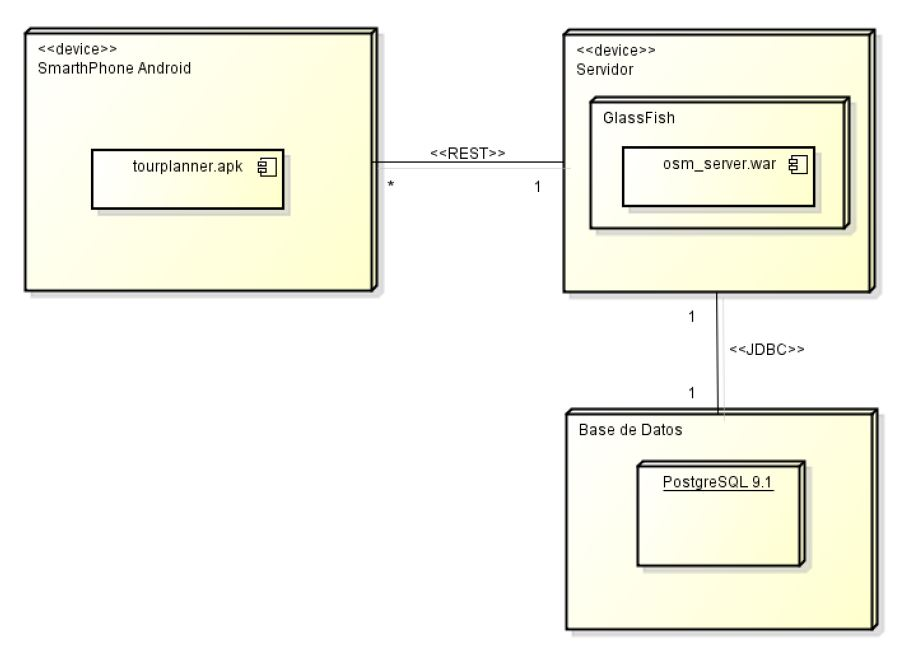
\includegraphics[width=\textwidth]{diagramaDespliegue.jpg}


\section{Diseño procedimental}

\subsection{Diagramas de secuencia}

\section{Diseño arquitectónico}

En este apartado se pueden ver los distintos patrones de diseño que han sido aplicados sobre el código para lograr una estructura mucho mas homogénea y reutilizable a futuro.

Como se comentó en el proyecto anterior, se aplicaron los patrones Singleton y Facade para dos partes distintas del desarrollo de la estructura del proyecto.

Por desgracia, el patrón Facade se implementó para acceder al servicio de Panoramio, el cual ya no se encuentra activo, por lo que objetivamente no se está poniendo en práctica real para este proyecto. De todas formas, es un patrón perfectamente válido y una vez localizada una API que pueda sustituir los servicios prestados por Panoramio, se podría volver a aplicar sin ningún problema.

El patrón Singleton se sigue utilizando para el manejo de la clase SSLFactory, ya que seguimos necesitando validar y asegurar que se está realizando una conexión HTTPS con el servidor y este patrón nos ayuda bastante para poder hacerlo de manera ordenada.



\apendice{Documentación técnica de programación}

\section{Introducción}

En este apartado de la memoria, nos centraremos en la parte más técnica del trabajo, entrando a detalle sobre los cambios realizados y los problemas diversos que se han encontrado y solucionado.

Mencionaremos algunas partes que hacen referencia al servidor, teniendo en cuenta que esta parte no la hemos desarrollado, ya que lo hizo mi compañero Ignacio.

Dentro de este apartado, veremos las distintas bibliotecas que se han utilizado, las APIs, el manual del programador y también las pruebas realizadas. 

Cabe destacar que en este proyecto la mayor parte de desarrollo ha sido sobre la resolución de errores provocados por el cambio de versión y la antigüedad del proyecto, sin poder mostrar implementaciones nuevas con respecto a funcionalidades. Es un trabajo dedicado al mantenimiento y actualización de una aplicación que contaba con una versión y recursos con 7 años de antigüedad y por eso ha habido tanta base de problemas.

Del mismo modo que hemos hecho en algunos apartados, se mencionarán partes que ya fueron desarrolladas anteriormente y que no hayan sufrido cambios importantes.

\section{Estructura de directorios}

En este apartado vamos a enumerar distintos contenidos que tendrá el dispositivo entregable, tanto del cliente como del servidor:

\begin{itemize}
\item Cliente
 	\begin{itemize}
		\item Aplicación: dentro de esta subcarpeta tendremos el archivo TourPlanner.apk, para que pueda ser instalado en cualquier dispositivo.
		\item Código fuente: Contiene el código de la aplicación Android.
		\item Javadoc: documentación sobre la aplicación.
		\item Datos: contiene el archivo con las referencias utilizadas en el proyecto y un backup con la base de datos PostgreSQL de Burgos configurada.
		\item Máquina virtual: Dentro tendremos la máquina virtual donde estará instalado Android Studio y se podrá utilizar sin tener que hacer más instalaciones.
		\end{itemize}
		
\item Servidor
 	\begin{itemize}
		\item Aplicación: contiene el archivo osm server.war para que se pueda utilizar en cualquier momento.
		\item Código fuente: Contiene el código fuente de la aplicación servidor.
		\item Javadoc: Contiene la documentación de la aplicación servidor.
		\item Datos: Archivo con las referencias utilizadas en el proyecto y un backup con la base de datos PostgreSQL de Burgos configurada.
		\item contiene la máquina virtual del servidor configurada para ser utilizada.
		\end{itemize}
		
\item Documentación Memoria
 	\begin{itemize}	
		\item PDF: Contiene la memoria en formato PDF.
		\item Latex: Contiene la memoria en formato de latex.
		\end{itemize}
		
\item Software
 	\begin{itemize}
		\item Esta carpeta contendrá los distintos programas que se han ido utilizando en el desarrollo de la aplicación.
		\end{itemize}		
\end{itemize}

\section{Manual del programador}

Dentro de este apartado veremos todo el proceso de desarrollo que se ha realizado en el proyecto, explicando los cambios, mejoras y arreglos sobre el mismo. Lo dividiremos en distintos puntos, ya que es necesario cubrir todos los aspectos que hacen referencia al desarrollo del código y de la aplicación.

Antes de comenzar, cabe destacar que en este proyecto se ha tratado de mejorar el código de una aplicación con una antigüedad de 7 años, actualizándola a versiones compatibles con los dispositivos de hoy en día y a su vez tratando de que sea lo más estable posible. Ha habido funcionalidades que no se han podido actualizar tal y como estaban desarrolladas, por lo que se mencionarán para un futuro desarrollo.

\subsection{Modificaciones sobre la estructura}

En este pequeño apartado mencionaremos las modificaciones que ha sufrido la estructura dentro de la herramienta de desarrollo, partiendo de la base de que la herramienta en sí es distinta y consideramos que para este propósito Android Studio consigue una estructura más clara y sencilla, donde se pueden localizar mejor las distintas partes de las que está compuesta la aplicación, porque está organizada de forma mas homogénea.

En el proyecto anterior contábamos con una estructura como la siguiente:

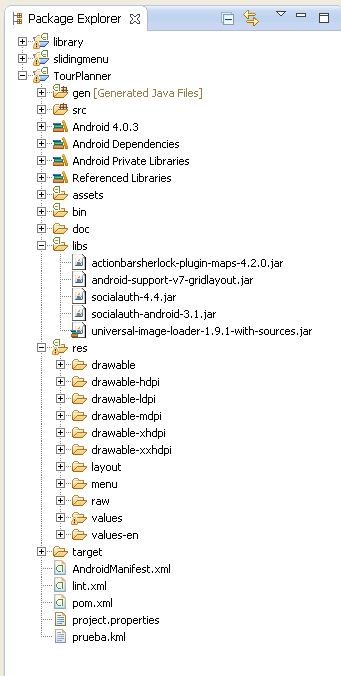
\includegraphics[width=\textwidth]{androidAnterior.jpg}

Aquí se puede observar que hay 3 carpetas principales:

\begin{itemize}
\item Tourplanner, la cual hace referencia a la aplicación. Dentro de esta carpeta esta la mayor parte del código de desarrollo y tambien se hace referencia a librerías y recursos.
\item SlidingMenu, que en este proyecto es la biblioteca utilizada para generar el menú lateral con el cuenta la aplicación. Como se puede ver es necesario que esté implementada de manera individual, en vez de ser importada como el resto de librerias y también tiene código dentro de sus subcarpetas.
\item libraries, que hace referencia a las librerías que estan utilizando en el proyecto, excepto SlidingMenu por lo que acabamos de ver.
\end{itemize}

Comparando esta estructura con la que tenemos actualmente podremos ver bastantes diferencias:

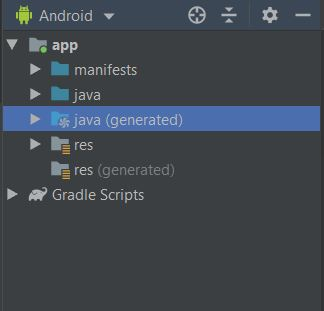
\includegraphics[width=\textwidth]{androidNuevo.jpg}

En este caso, podemos ver una estructura mas sencilla, ya que sólo contamos con una carpeta principal de la que aparecen el resto de elementos. 

La carpeta java, que será donde se encuentre todo el código de desarrollo de la aplicación. No tendremos que estar desplazandonos entre otros directorios para poder encontrar código, ya que estará al completo aquí.

\subsubsection{Gradle Scripts}

Por otro lado, el apartado de Gradle Scripts es algo que Android Studio implementa por defecto en todos los proyectos, y es una herramienta muy útil cuando se trabaja con un numero considerable de librerias, pudiendo manejar a la perfección qué se está importando para que sea utilizado, así como las versiones en las que lo implantamos.

El hecho de poder manejar las versiones de esta manera nos permite poder mantener la aplicación lo más actualizada posible continuamente, ya que además el propio Software nos advertirá siempre que tengamos versiones de repositorios para los cuales ya hay otras más nuevas. Esto ayuda a mantenerse siempre lo más alejado posible de trabajar con "bujs" y errores de desarrollo de los propios repositorios, ya que suele ser lo que se corrige cuando se actualiza el Software.

El fichero más importante del apartado de Gradle será el llamado "build.gradle", ya que será con el que podremos añadir repositorios y bibliotecas para que despues podamos implementar en el código.

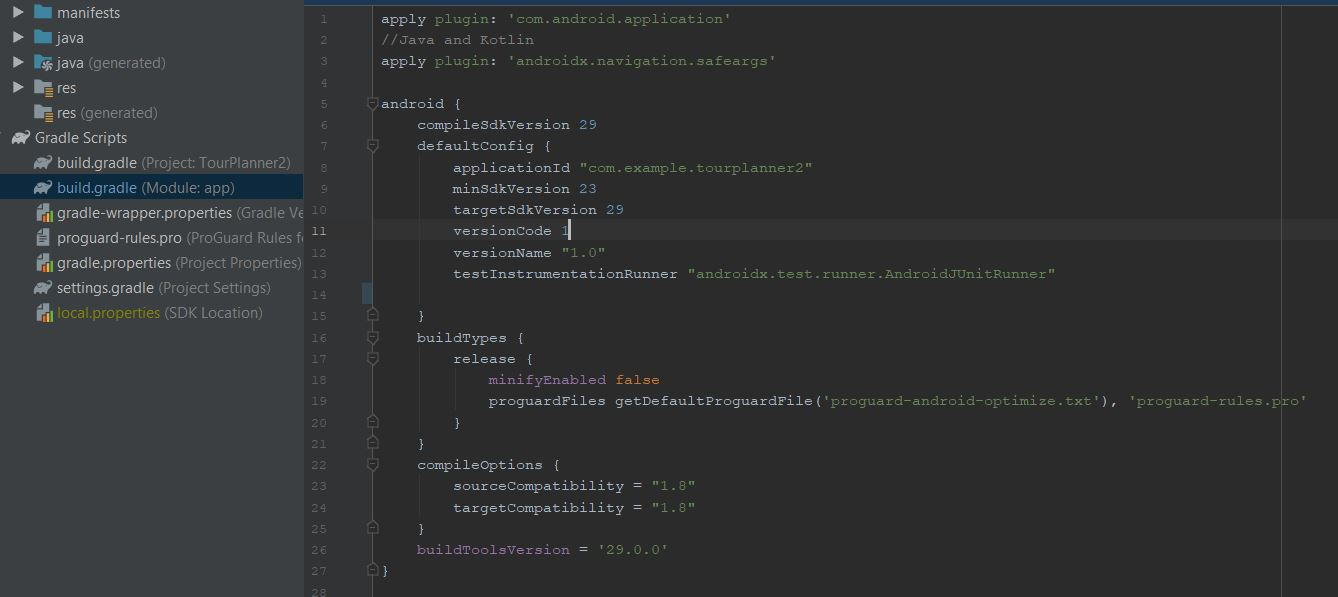
\includegraphics[width=\textwidth]{gradle1.jpg}

Como se puede observar, aquí configuraremos la versión de sdk con la que estamos trabajando y la versión mínima con la que podremos hacer funcionar la aplicación. La versión mínima será la API 23, como se indica en esta configuración y la versión objetivo que se menciona aquí también será la API 29, que es la última con la que cuenta Android. Nuestra aplicación funcionará para dispositivos con versión Android 6.0 (API 23) o superior.

Por último podemos ver cómo nos recomienda Android que mantengamos actualizado nuestro software y repositorios, ya que en el momento que alguno de ellos tiene una versión disponible superior, nos los marcará:

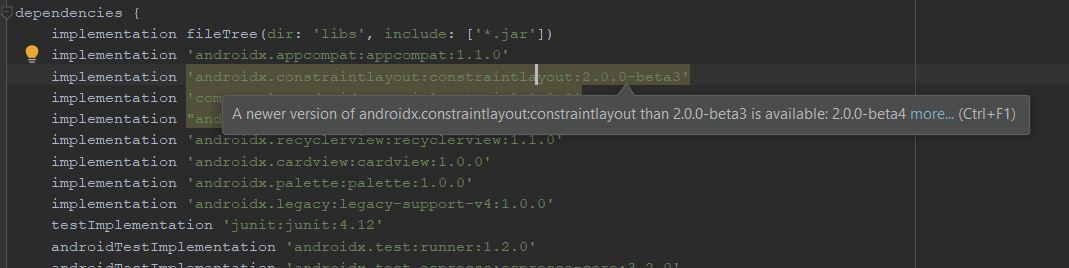
\includegraphics[width=\textwidth]{gradleVersion.jpg}

\subsection{Modificaciones importantes sobre bibliotecas}

Como ya hemos mencionado en otros apartados de la memoria, se han realizado muchas modificaciones sobre las librerías que estaban siendo utilizadas previamente y que, por desgracia, han quedado totalmente obsoletas. Esto nos ha llevado a intentar descubrir todas las novedades que se han ido implementando en el software de Android desde el desarrollo del anterior proyecto.

\subsubsection{Cambio de SlidingMenu}

Uno de los primeros descubrimientos que nos vimos obligados a realizar fue el de una nueva herramienta par obtener el menú "deslizante" con el que contaba la aplicación, o al menos un nuevo menú que cumpliera la función que ya cumplía previamente SlidingMenu.

Esto se debe a que la librería de SlidingMenu quedo obsoleta, y no se siguió desarrollando soporte para la misma a lo largo de las nuevas versiones, por lo que al intentar utilizarla en Android Studio con la versión para la API 23, ésta no era reconocida.

De esta forma, hemos desarrollado el nuevo menú de la aplicación, utilizando una versión más estándar proveniente de Android, lo cual nos asegurará más soporte de cara a futuro y es mucho menos probable que tenga que ser sustituida por completo en una futura versión. El menú en cuestión es NavigationMethod y es una funcionalidad de la biblioteca de androidx, la cual ha sido utilizada en muchas partes de este proyecto. Éste menú nos ofrece una funcionalidad muy parecida a lo que ya nos encontrábamos antes, pero mejorando la eficiencia y la visualización, siendo esta última bastante más parecida a la que nos podemos encontrar en cualquier dispositivo que utilice Android. Esto también ayuda a la accesibilidad de cara al usuario.

La interfaz del menú que teníamos antes era de esta forma:

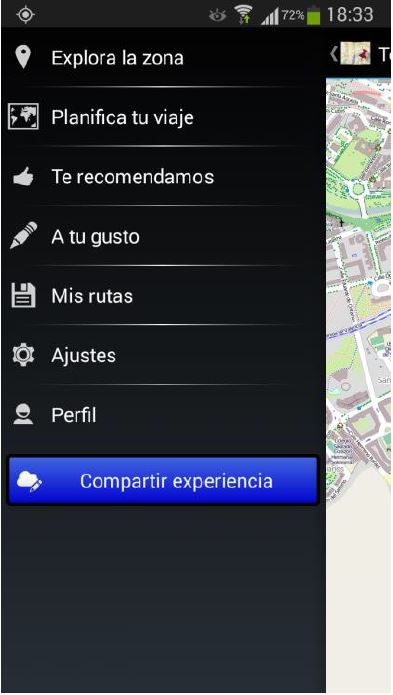
\includegraphics[scale=1]{interfazVieja.jpg}

La interfaz del menú que tenemos ahora es de la forma:

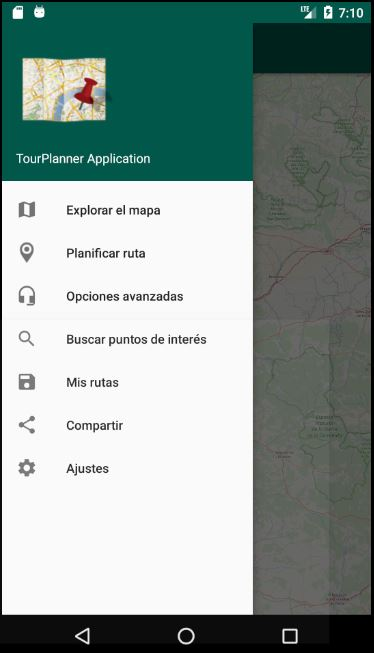
\includegraphics[scale=1]{interfazNueva.jpg}

Como podemos ver, hay un cambio considerable, tanto en facilidad a la hora de visualizarlo, como de desarrollarlo en código, ya que implementar este menú, al ser un estándar de Android, nos resulta una tarea más accesible y en caso de tener dudas, también es mas sencillo conseguir documentación al respecto. Estas son las ventajas que nos ofrece estar utilizando repositorios estándar para Android.

Las dos bibliotecas que han sustituido a SlidingMenu han sido:

\begin{itemize}
\item NavigationMethod, y los métodos que implementa.
\item Android.view.Menu
\end{itemize}

También los colores es algo en lo que se ha puesto cierta atención a la hora de desarrollar este menú y el resto de la aplicación, ya que consideramos que la accesibilidad de una aplicación hoy en día es un valor añadido muy importante. Se ha tratado de manejar colores que faciliten a la lectura y visualización, siguiendo los estándares de accesibilidad de W3C.

\subsubsection{Librería SherlockActivity}

Esta es otra de las bibliotecas que más han afectado al desarrollo, ya que la mayoría de "activities" estaban construidas en torno a ella. Como Ocurrió con SlidingMenu, también  nos encontramos con que la biblioteca estaba "deprecated" u obsoleta pero, por desgracia, no se había continuado el desarrollo de la misma y por lo tanto no era una cuestión de actualizar a una versión más actualizada, porque ésta no existía. Por esto mismo se tuvo que buscar una alternativa y pasar a utilizar algo más estandarizable, siempre evitando que en un futuro suceda algo similar a lo que nos ha sucedido a nosotros.

Así fue como se comenzó a implementar la librería de AppCompatActivity, pero no en todas las actividades que conformaban la aplicación, sino en la principal. Para poder explicar esto es necesario mencionar la libreria anterior de NavigationMethod, ya que en este sentido se ha conseguido solucionar los dos problemas utilizando un método estándar que está más optimizado para el manejo de aplicaciones como la nuestra, donde se maneja un número considerable de ventanas diferentes y estas poseen comunicación e interacción.

Hablamos del concepto de Activity y Fragment.

\begin{itemize}
\item Activity. Se podría definir como una ventana de la aplicación. En código corresponde a una clase de Java, que contiene todos los métodos que sirva para mostrar información, aunque por otro lado la parte más visual corresponde a un archivo .xml que será el que contenga la información puramente visual, configuración de colores, tamaños, etc.
\item Fragment. A efectos visuales contiene lo mismo que una Activity, pero en este caso la verdadera diferencia surge en la comunicación entre ellas y la optimización de la aplicación en cuanto a tiempos a la hora de navegar entre ventanas. Por otro lado, para implantar correctamente el menú del que hablábamos en el punto anterior, la manera más óptima es tenerlo instaurado dentro de una activity, y que los distintos apartados (ventanas) que tengamos dentro de ese menú sean Fragment. De esta forma conseguimos navegar desde una ventana principal hacia el resto de apartados utilizando el NavigationView.
\end{itemize}

\subsubsection{Librería Org.Apache}

La última de las bibliotecas mas conflictivas a la hora de desarrollar la aplicación ha sido la de Org.Apache. Esto se debe principalmente a que, como las dos anteriores supone una carga dentro del código bastante grande, pero a diferencia de estas no obtenemos un error directo por su parte a la hora de implantarlo en nuestro codigo actualizado, sino que obtuvimos los problemas más adelante.

De hecho, pese a que estuviera obsoleta, se decidió que en un principio no se modificaría, ya que suponía un cambio excesivamente grande y costoso como para invertir recursos en algo que aparentemente en un inicio funionaba correctamente. Finalmente no se ha podido recurrir a otra opción, ya que hay métodos de esta biblioteca que no dan el resultado esperado a la hora de ejecutar todo el código.

El problema principal es que supone un cambio en todas las clases donde se realiza una petición de tipo HTTP o HTTPS, ya que son éstas la que utilizan los métodos provenientes de Org.Apache. 

Los metodos que más utilizados estaban siendo eran:

\begin{itemize}
\item DefaultHttpClient. Éste es con diferencia el método que más implementaciones y llamadas recibía dentro de las clases de la aplicación. Era el método que servía para iniciar la conexión HTTP.
\item HttpsClient. Ésta clase había sido implementada por los desarrolladores anteriores del proyecto y aportaba la posibilidad de realizar una conexión HTTPS o lo que es lo mismo, una conexión segura a través del protocolo SSL. El problema es que también dependía al completo de métodos obsoletos.
\end{itemize}

Finalmente, se consiguió aplicar otro cambio importante, también hacia la estandarización, ya que se han modificado todos los métodos y llamadas dentro de clases para que pasen a utilizar HttpsUrlConnection, que es la librería estándar de Android que nos ofrece el desarrollo y manejo de peticiones y conexiones HTTPS.

Para realizar la conexión utilizando esta librería tendremos que seguir unos pasos mas sencillos que antes, aunque por otro lado bastante similares.

\begin{itemize}
\item Establecemos una direccion URL, que nos servirá para poder alcanzar el destino de nuestras peticiones.
\item Instanciamos la conexión de tipo HttpsUrlConnection, utilizando la URL mencionada.
\item Establecemos todos los parámetros que consideremos necesarios para poder establecer la conexión, como por ejemplo el tiempo de "Timeout" para poder conectarnos y evitar malgasto de recursos.
\item Una vez está todo lo anterior configurado, simplemente realizamos la conexion a traves del método connect().
\item por ultimo quedaría recibir respuesta, lo cual podremos obtenerlo con metodos como getResponseCode(), obteniendo la respuesta que hayamos recibido de parte del servidor, y pudiendo enviar nuevas peticiones en base a esta respuesta.
\end{itemize}

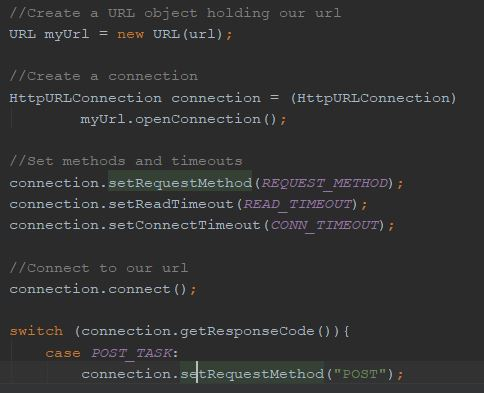
\includegraphics[scale=1]{codigoHTTPS.jpg}

Como se puede ver en la imagen, realizar esta conexión supone bastante poca carga de código y al ser un método bastante parecido, si se utiliza varias veces en una misma clase, se podría realizar EXTRACT METHOD sobre varias partes, para evitar aun más la sobrecarga de código.

\subsection{Cambios sobre APIs}

En este caso, hablaremos sobre las APIs que antes eran utilizadas, pero con el motivo de haber quedado obsoletas, no ha sido posible seguir contando con su funcionalidad dentro de la aplicación.

\subsubsection{Panoramio}

Una de ellas es Panoramio, que nos proveía de imágenes para que fueran mostradas dentro de los detalles de un punto de interés. Desde que este proyecto Online fue absorvido por Google, ya no podemos contar con el servicio de obtención de imágenes gratuito y por tanto la API que nos permitía hacerlo ha ido quedando en el olvido, al no tener más sentido de existencia.


\includegraphics[width=\textwidth]{panoramio.jpg}

\section{Compilación, instalación y ejecución del proyecto}

En este apartado se cubrirá todos los aspectos referentes a la utilización de la aplicación, por lo tanto veremos cómo instalar todo el software necesario, cómo compilar el proyecto de Android y tambien cómo ejecutarlo.

Cabe destacar que sólo se va a cubrir la instalación, compilación y ejecución de la aplicación de Android, ya que la parte referente al servidor se tratará en detalle en el proyecto de mi compañero Ignacio.

\subsection{Instalación}

Las herramientas que vamos a necesitar tener instaladas por parte de la aplicación Android serán, básicamente Android Studio y sus componentes internos. Vamos a observar cómo lo instalaremos.

\subsubsection{Android Studio}

Simplemente necesitaremos acceder a la página oficial de Android, a traves del siguiente enlace (), y veremos lo siguiente:

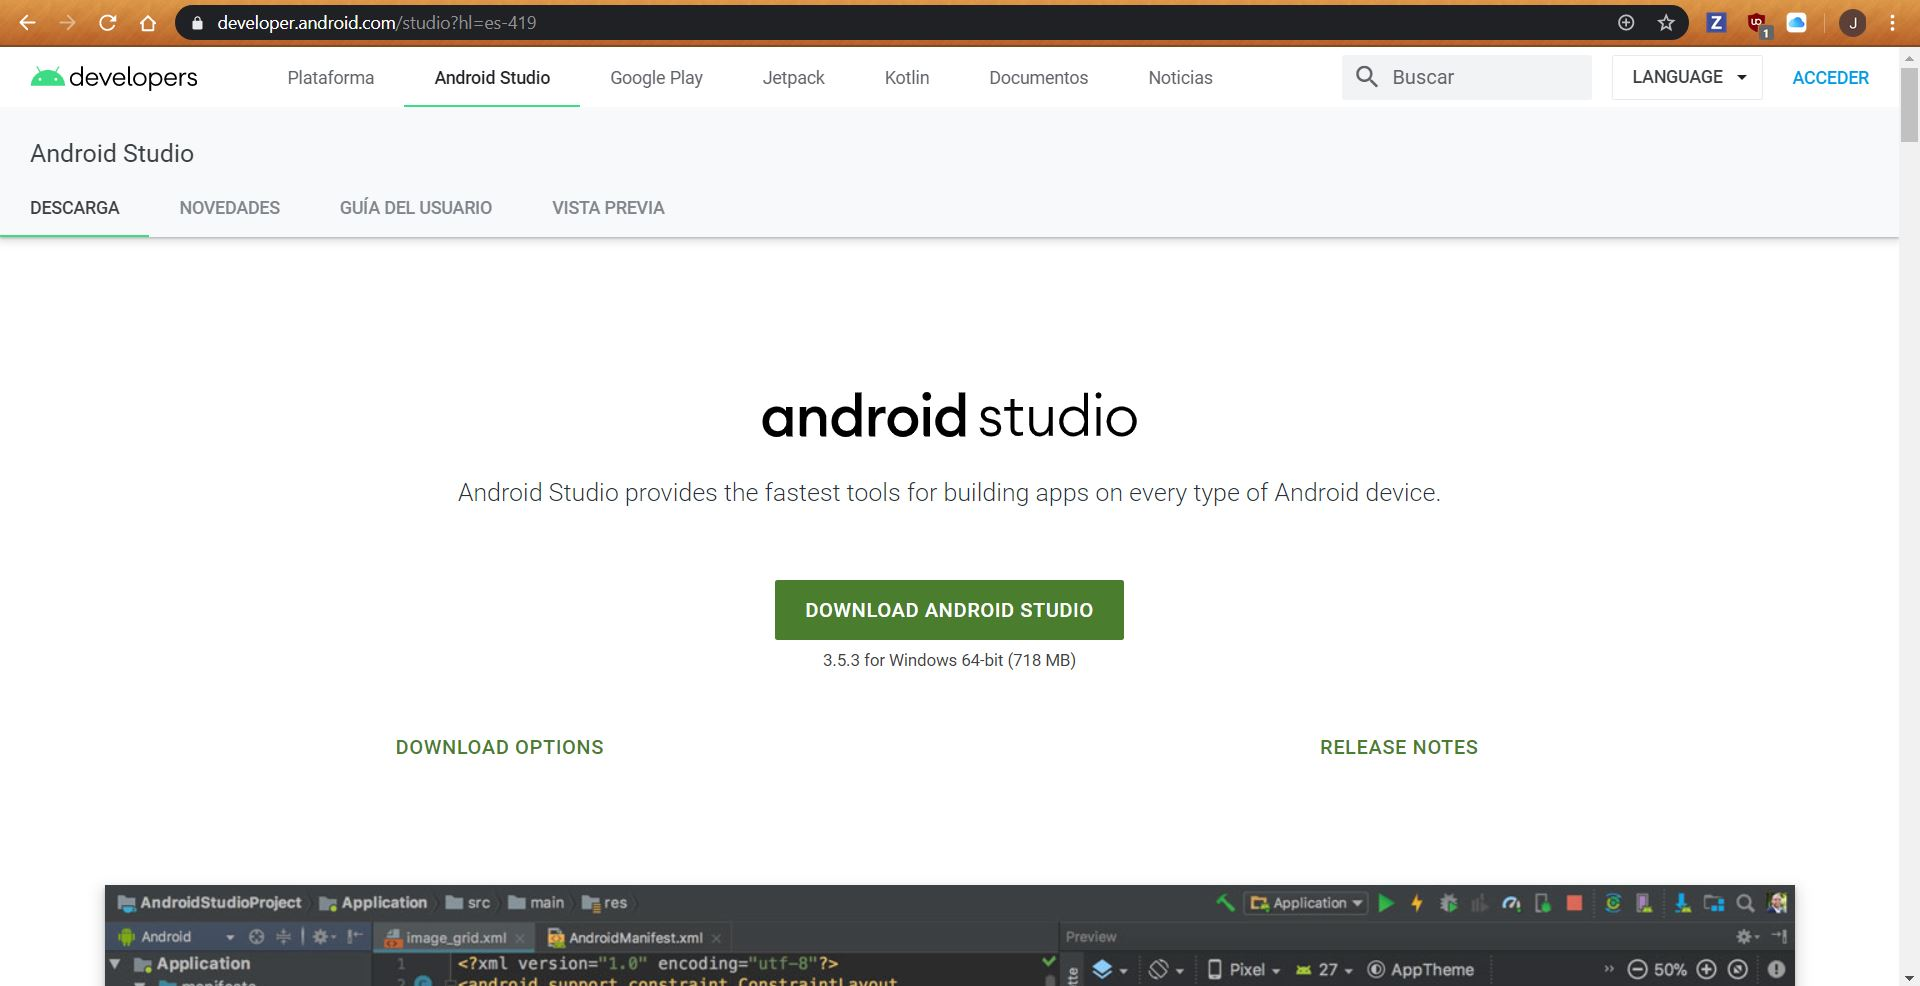
\includegraphics[width=\textwidth]{androidInstala.jpg}

Cómo se puede observar, bastará con pulsar la opción para descargar Android Studio. En esta opción siempre nos ofrecerá la última versión oficial del producto. Excepto en casos excepcionales, esto es lo más recomendable, ya que al ser un software que exige bastantes recursos, cuanto más actual sea la versión que estamos utilizando mejor optimizada estará. 

Si se da uno de los casos excepcionales que mencionábamos, también nos ofrecen diferentes versiones o incluso diferentes sistemas operativos con los que son compatibles.

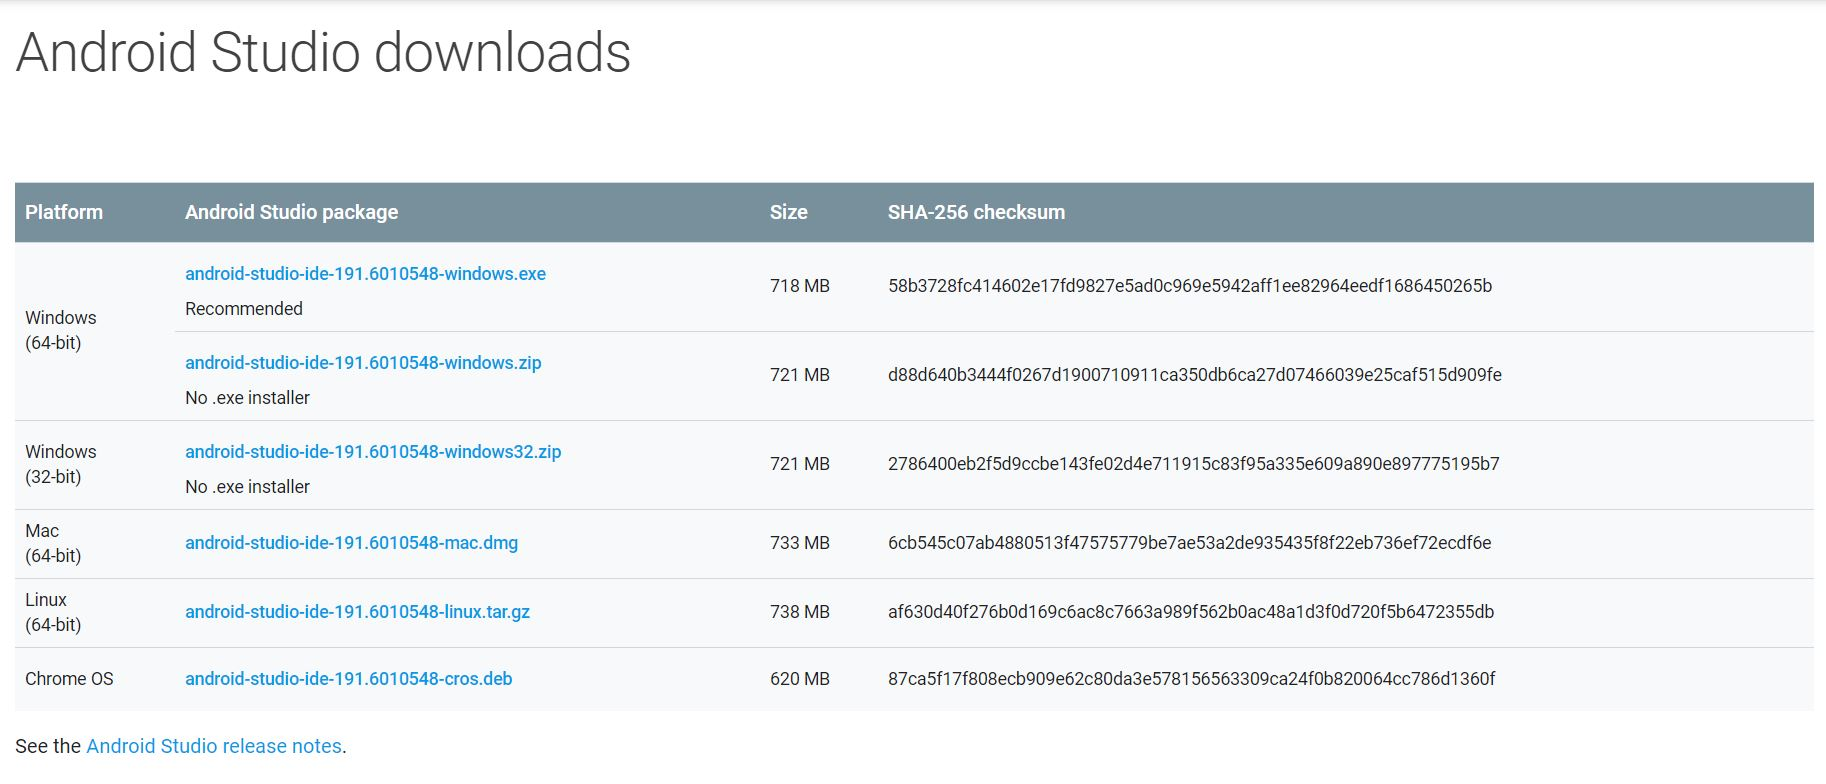
\includegraphics[width=\textwidth]{androidVersiones.jpg}

Como se puede observar, también nos ofrecen la opción de acceder a las "release notes", lo cual resulta muy útil para poder descubrir más a fondo los cambios que se han desarrollado en cada versión.


\subsubsection{SDK Manager}

Esta herramienta es parte de Android Studio, pero necesitaremos configurarla por separado, para poder contar después con una experiencia fructífera:


\includegraphics[scale=1]{sdkManager.jpg}

Una vez pulsemos ese botón remarcado en rojo, entraremos en la configuración del SDK Manager:

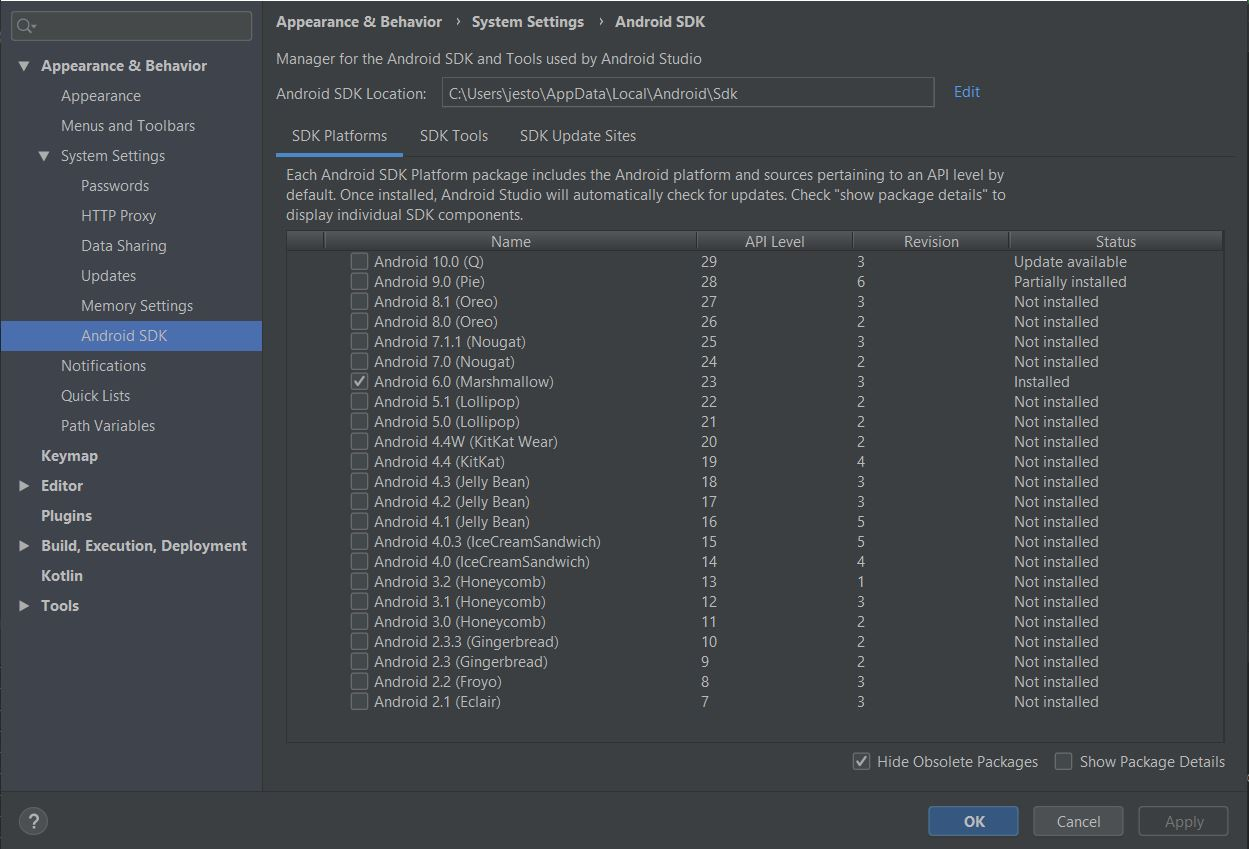
\includegraphics[width=\textwidth]{sdkVersiones.jpg}

Como podemos ver, la primera ventana que nos ofrece este gestor, será para que seleccionemos la versión de Android sobre la que queremos trabajar en nuestor proyecto. Como ya hemos mencionado previamente, nosotros tenemos instalada la versión de Android 6.0.

También contamos con otras dos ventanas:

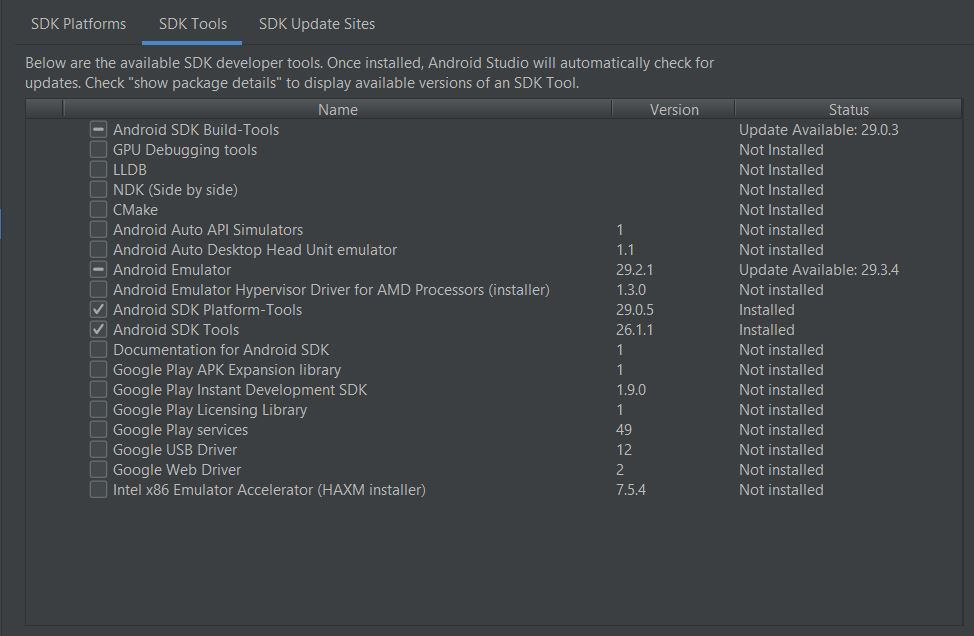
\includegraphics[width=\textwidth]{sdkCosas.jpg}

Dentro de esta segunda ventana podremos configurar las herramientas adicionales que instalaremos para conseguir una mejor experiencia mientras desarrollamos las aplicaciones. En nuestro caso, tenemos instalado el emulador, que resulta totalmente necesario para hacer pruebas.

Por último contamos con la ventana de actualizaciones:

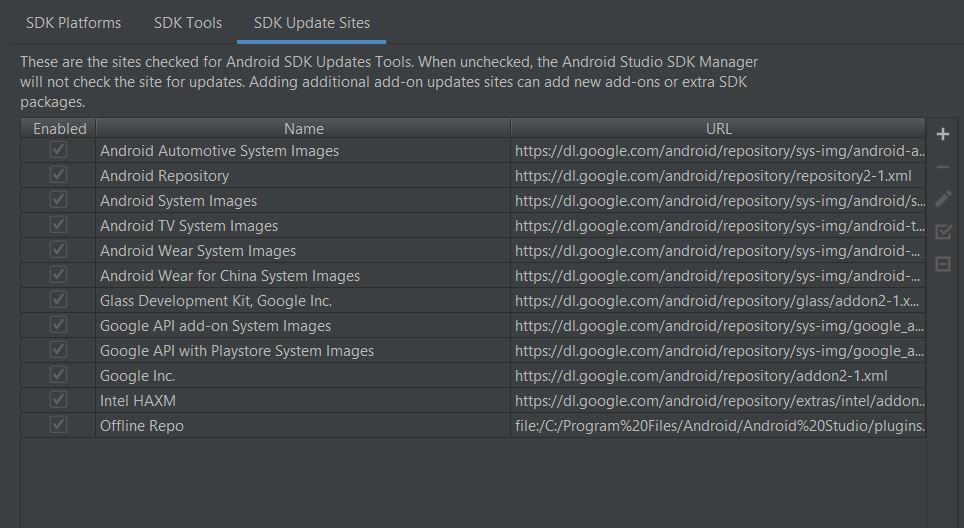
\includegraphics[width=\textwidth]{sdkUpdate.jpg}

En esta ventana, tal como se describe, se podrá configurar los repositorios de los que se realizarán comprobaciones en busca de actualizaciones de manera automática.

\subsubsection{AVD Manager}

Este gestor será el que nos permita llevar un control sobre el emulador de Android, ya que aquí será donde instalaremos el dispositivo móvil virtual que después ejecutaremos para probar nuestra aplicación.


\includegraphics[scale=1]{avdManager.jpg}

Una vez pulsemos tendremos acceso a la configuracion de nuetros dispositivos virtuales:

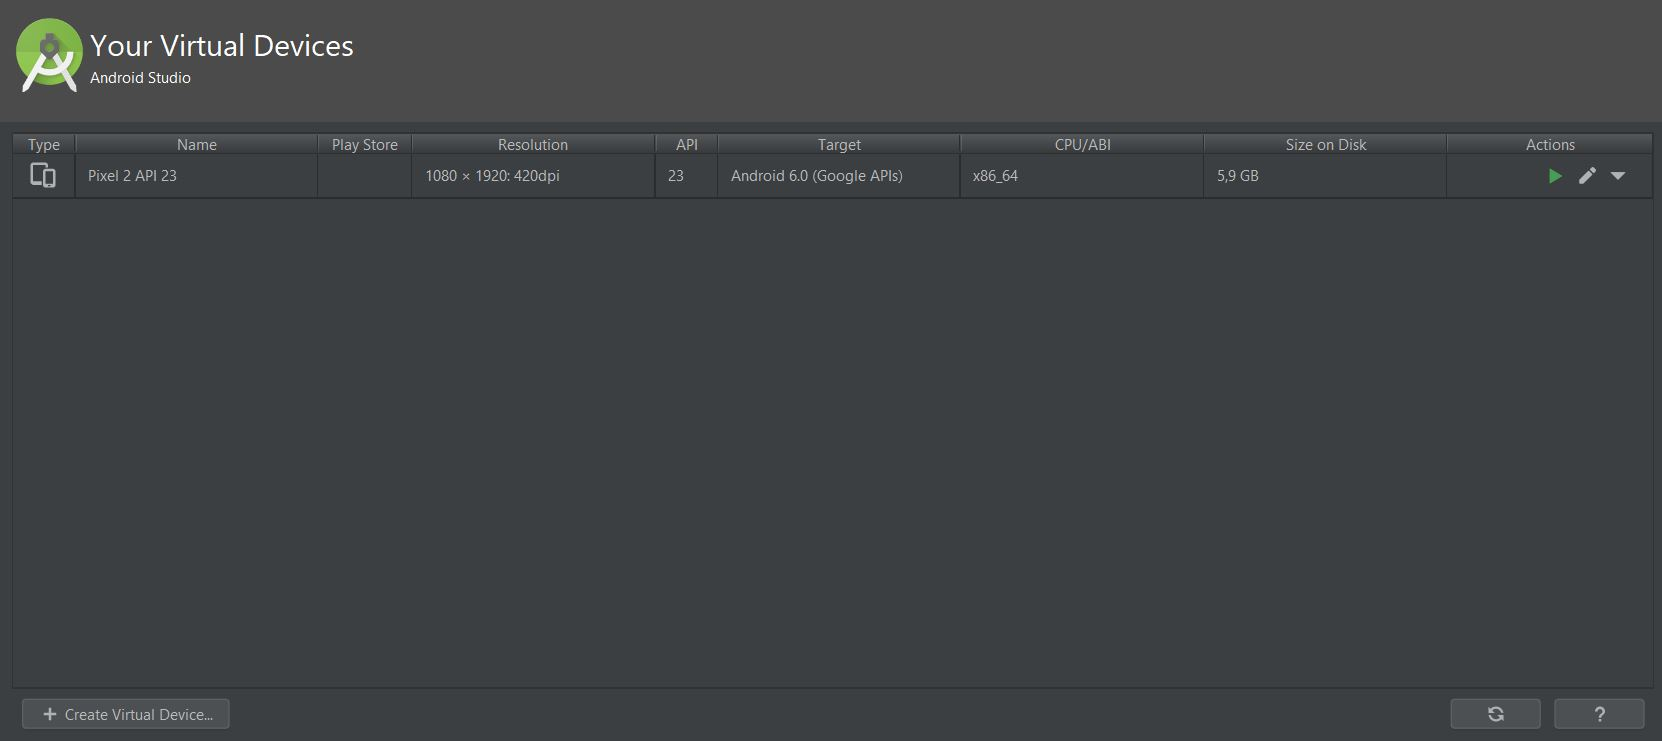
\includegraphics[width=\textwidth]{avdPrincipal.jpg}

Aqui ya podremos ver los dispositivos que tenemos instalados, ejecutarlo, eliminarlos o modificar algunas configuraciones.

Si queremos crear un dispositivo tendremos que seleccionar el botón de "Create Virtual Device":

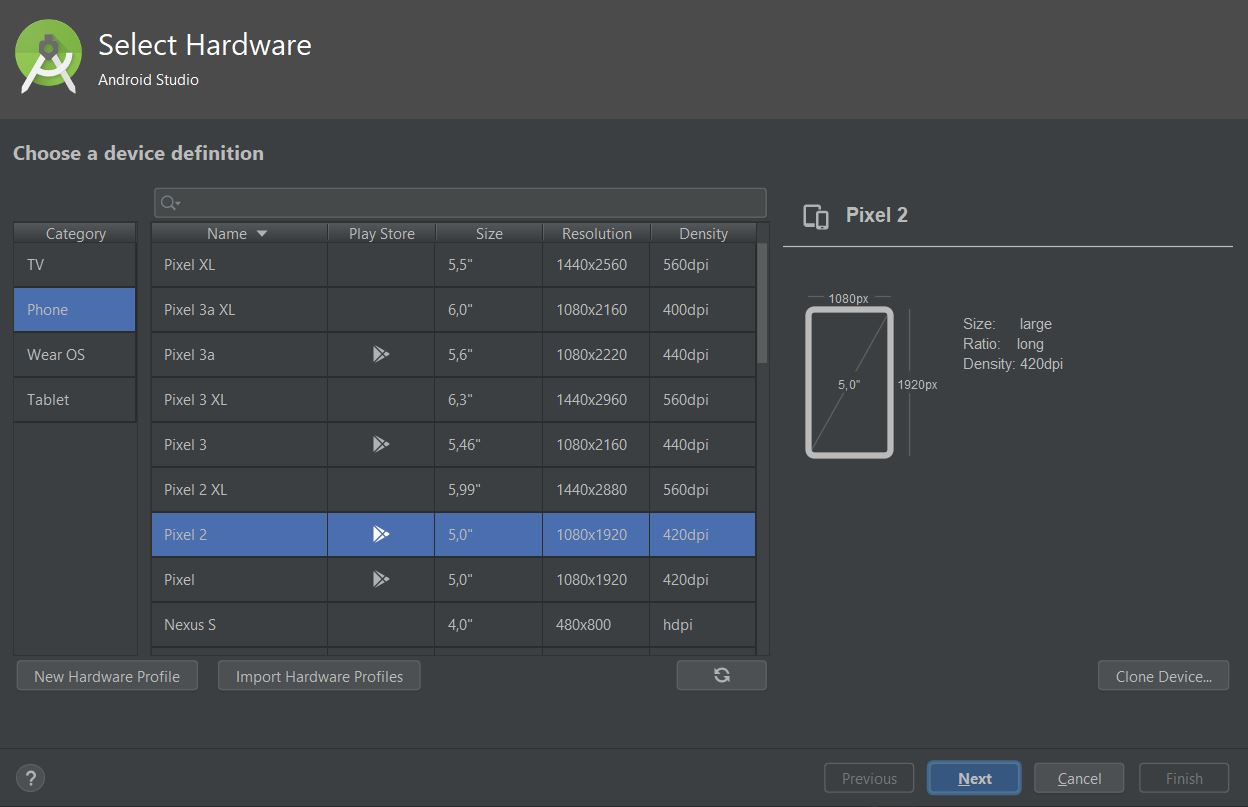
\includegraphics[width=\textwidth]{avdNuevo.jpg}

En esta ventana simplemente seleccionaremos que modelo de dispositivo móvil queremos simular, descargarlo y utilizarlo.

\subsection{Compilación}



\subsection{Ejecución}

\section{Pruebas del sistema}

\apendice{Documentación de usuario}

\section{Introducción}

Dentro de este anexo se podrán ver los requisitos HardWare y SoftWare que tiene la aplicación para poder ser funcional, así como un manual de usuario para que cualquiera que decida usar esta aplicación tenga una guía sencilla que pueda utilizar.

\section{Requisitos de usuarios}

\subsection{Requisitos HardWare}

Para poder realizar una ejecución correcta de la aplicación se necesitará utilizar un emulador de Android que esté instalado en un ordenador con un rendimiento bastante alto, ya que este tipo de programas para emular un sistema Android al completo, exigen muchos recursos de CPU y RAM.

Otra exigencia básica para poder hacer funcionar el emulador de Android Studio es que la CPU cuente con estos requisitos mínimos:

\begin{itemize}
\item SDK Tools 26.1.1 o versiones posteriores.
\item Procesador de 64 bits.
\item CPU con compatibilidad para UG (invitado no restringido)
\item HAXM 6.2.1 o posterior (se recomienda HAXM 7.2.0 o posterior)
\item También se ha observado que en cuanto al tipo de procesador, en el caso de intel no causa ningún problema, pero con AMD, parece que sólo lo soportan los procesadores más nuevos. Esto fue probado en un procesador AMD Ryzen 2700x y no fue capaz de ejecutar el programa de emulador, en cambio en un procesador intel i7 de 8th generación funciona a la perfección.
\end{itemize}

Por supuesto, también cabe destacar que otra forma de hacer que la aplicación funcione, tratándose de Android, es usar un dispositivo que tenga una version instalada de Android 6.0 o superior. De esta manera podremos observar cómo es la experiencia al completo de ésta aplicación en un dispositivo real. 

La aplicación ha sido instalada en un dispositivo móvil Google Pixel 2 a través del emulador y en un BQ Aquaris E5 de manera física. Ambos funcionaron a la perfección bajo los requisitos mencionados anteriormente.  

\subsection{Requisitos SoftWare}

Estos son los requisitos software:

\begin{itemize}
\item Compilador de Java. Servirá para poder programar la aplicación de Android y también para ejecutar la maquina virtual Java.
\item Android Studio, ya que esta nueva herramienta proporcionada por Google permite desarrollar la aplicación en un entorno totalmente compatible. También ofrece numerosos tooltips a la hora de programar.
\item Android Developer Tools. Ésta herramienta viene incorporada en Android Studio y supone la base para poder desarrollar todo el código de Android.
\item Oracle GlassFish Server 3.0, que contendrá el servidor encargado de las respuestas al cliente.
\item Oracle VM VirtualBox, el cual servirá si no queremos instalar los programas mencionados, ya que con tenerlo todo listo en una maquina virtual podríamos ejecutar el cliente o servidor desde allí. Es importante mencionar que será necesario un ordenador con bastante potencia para poder aprovechar esta opción.
\end{itemize}

\section{Instalación}

En esta sección se encuentra detallada la guía de instalación de la aplicación.

Cabe destacar que es necesario instalar tanto el cliente en un dispositivo Android (o emulador) como el servidor en GlassFish.

\subsection{Instalación de la aplicación servidor}

Debido a que la versión de GlassFish utilizada es la misma que en anteriores versiones del proyecto, se seguirán los mismo pasos para la instalación del servidor. Dichos pasos son los siguientes:

Para instalar la aplicación en el servidor, hay que abrir la consola de administración de GlassFish tecleando en un navegador web la dirección del servidor con el puerto 4848 (http://localhost:4848 en este caso) e ir a la opción Applications.

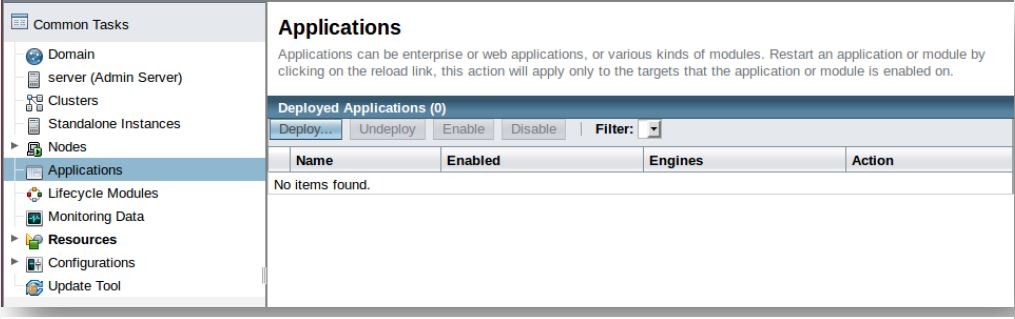
\includegraphics[width=\textwidth]{instalacionServer1.jpg}

A continuación hay que hacer click sobre el botón Deploy e indicar la ruta en la que se encuentra el archivo "osm server.war". Después, hacemos click sobre el botón OK y ya tendremos la aplicación publicada y funcionando.

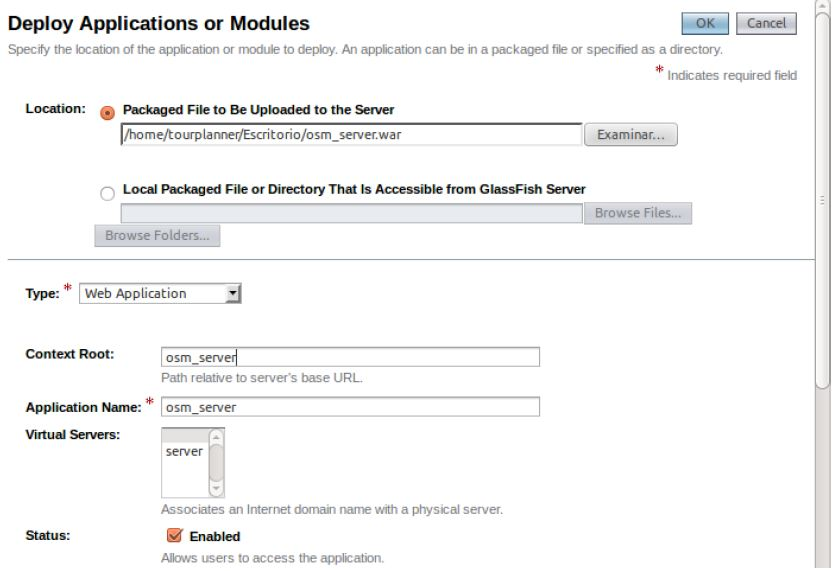
\includegraphics[width=\textwidth]{instalacionServer2.jpg}

\subsection{Instalación de la aplicación cliente}

Para realizar la instalación de nuestra aplicación Android en un dispositivo físico o un emulador, es necesario seguir estos pasos:

\begin{itemize}
\item Se necesitará, en caso de un dispositivo físico, tenerlo conectado al ordenador en el que estamos desarrollando la aplicación.
\item Una vez esté lista la aplicación, bastará con pulsar el botón de "play" en Android Studio.

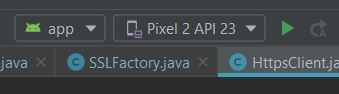
\includegraphics[width=\textwidth]{playAndroid.jpg}

\item Android Studio será el encargado de instalar el archivo.apk dentro del dispositivo y lo ejecutará directamente.
\end{itemize}


\includegraphics[width=\textwidth]{installAndroid.jpg}

Hay que tener en cuenta que para el correcto funcionamiento de la aplicación hay que seguir correctamente los pasos de compilación explicados en el apartado "Compilación del cliente", prestando especial atención al punto en el que se establece la dirección IP y puerto del servidor.

\subsection{Ejecución de la aplicación}

Para lograr que la aplicación servidor se ejecute sin la necesidad de contar con un servidor y un cliente independientes se han incluido en el USB del proyecto las maquinas virtuales correspondientes al cliente y servidor. De esta forma podremos ejecutar la aplicación con un solo ordenador.

Una de las máquinas virtuales es windows 10 y para poder ejecutar el emulador de Android, será necesario que el ordenador en el que se esté compilando posea bastante potencia, además de cumplir los requisitos mencionados en la instalación de Android Studio.

Cabe destacar que para lograr que ambas máquinas virtuales se comuniquen entre sí correctamente, se ha utilizado el programa Logmein Hamachi que nos permite crear redes virtuales entre ambas máquinas a través de Internet.

\subsubsection{Ejecución de la aplicación servidor}

Para ejecutar la aplicación servidor, hay que importar la máquina virtual Servidor - Ubuntu 18.04 LTS en un software de virtualización como VirtualBox y ejecutarla.

Una vez iniciada, introducimos la contraseña tourplanner y ejecutamos el script startGlassfish que se muestra en la ilustración, con lo que a aplicación estará ejecutándose y escuchando a la espera de peticiones.



\subsubsection{Ejecución de la aplicación cliente}

Para ejecutar la aplicación cliente, al igual que la aplicación servidor, hay que importar la máquina virtual Cliente - Windows 10 en un software de virtualización como VirtualBox y ejecutarla.

Una vez iniciada, hacer doble click sobre el acceso directo del entorno de desarrollo Android Studio. A continuación, hacemos click sobre el icono "play". Después de esto se abrirá el emulador de Android con la aplicación instalada.

\section{Manual del usuario}

En este apartado se explicará las funcionalidades que posee la aplicación, para que en un momento dado resulte más cómodo para el usuario a la hora de ser utilizada. Es importante mencionar que algunos aspectos más relacionados con pantallas en las que se establezca conexión con el servidor no se mostrarán aquí, ya que son explicaciones que ya se han desarrollado de una forma bastante completa en anteriores trabajos \cite{tfm1} y en este caso el foco se pondrá sobre los cambios de interfaz y la funcionalidad más general.

Cuando el usuario inicie la aplicación, obtendrá la siguiente pantalla:

\imagen{fotoMapa}{Imagen inicial de la aplicación al iniciarse}

Si el GPS está activado, se utilizará este servicio para determinar el foco de la aplicación. Para poder hacer esto, la aplicación solicitará permiso al dispositivo.

Si no se dispone de GPS, hay una ubicación escrita por defecto.

Tras haber accedido a esta primera pantalla, si el usuario pulsa en el botón que está arriba a la izquierda o simplemente desliza el dedo de izquierda a derecha, podrá ver el menú de opciones con el que cuenta la aplicación:

\imagen{fotoMenu}{Imagen del menú de la aplicación}

Si el usuario pulsa en la opción de Explorar el mapa:

\imagen{fotoExplorar}{Imagen de la ventana Explorar el mapa}

Aquí podrá seleccionar entre las opciones que se ofrecen, y después al pulsar en \textit{Explorar}, accederá al mapa de nuevo con las modificaciones que se han hecho tras poner estas opciones.

También se puede ver la ventana de Planificar ruta:

\imagen{fotoPlanifica}{Imagen de la ventana de Planificar ruta}

Aquí, parecido a la anterior, se podrá configurar lo que se necesite y planificar la ruta.

Si el usuario necesita cambiar alguna configuración, tendrá que acceder a la ventana de Opciones:

\imagen{fotoOpciones}{Imagen de la ventana Opciones}

Una vez aquí dentro, se pueden configurar las formas de calcular las rutas, así como las distintas preferencias que se tienen sobre ciertos puntos de interés. Pudiendo hacer que no se tengan en cuenta los que se desmarquen.

Distintas opciones sobre la forma de calcular:

\imagen{fotoOpcionesAlgo}{Imagen de la selección de Aloritmos para calcular rutas}

También la interfaz al modificar ciertas clasificaciones de puntos de interés:

\imagen{fotoOpciones2}{Imagen de las opciones de marcado sobre los puntos de interés}

El usuario también puede acceder a la parte de \textit{Mis rutas}, donde podrá almacenar rutas que le hayan gustado y cargar algunas que ya tenga almacenadas. Para poder hacer esto será necesario estar identificado.

\imagen{fotoMisrutas}{Imagen de la ventana de Mis rutas}

Por último, se puede ver las opciones que ofrece la aplicación si se decide pulsar sobre \textit{Compartir}:

\imagen{fotoRedes}{Imagen de la selección de redes sociales al compartir}


\bibliographystyle{plain}
\bibliography{bibliografiaAnexos}

\end{document}
